\documentclass[11pt,a4paper,twoside]{book}
\usepackage[]{graphicx}\usepackage[]{color}
%% maxwidth is the original width if it is less than linewidth
%% otherwise use linewidth (to make sure the graphics do not exceed the margin)
\makeatletter
\def\maxwidth{ %
  \ifdim\Gin@nat@width>\linewidth
    \linewidth
  \else
    \Gin@nat@width
  \fi
}
\makeatother

\definecolor{fgcolor}{rgb}{0.345, 0.345, 0.345}
\newcommand{\hlnum}[1]{\textcolor[rgb]{0.686,0.059,0.569}{#1}}%
\newcommand{\hlstr}[1]{\textcolor[rgb]{0.192,0.494,0.8}{#1}}%
\newcommand{\hlcom}[1]{\textcolor[rgb]{0.678,0.584,0.686}{\textit{#1}}}%
\newcommand{\hlopt}[1]{\textcolor[rgb]{0,0,0}{#1}}%
\newcommand{\hlstd}[1]{\textcolor[rgb]{0.345,0.345,0.345}{#1}}%
\newcommand{\hlkwa}[1]{\textcolor[rgb]{0.161,0.373,0.58}{\textbf{#1}}}%
\newcommand{\hlkwb}[1]{\textcolor[rgb]{0.69,0.353,0.396}{#1}}%
\newcommand{\hlkwc}[1]{\textcolor[rgb]{0.333,0.667,0.333}{#1}}%
\newcommand{\hlkwd}[1]{\textcolor[rgb]{0.737,0.353,0.396}{\textbf{#1}}}%
\let\hlipl\hlkwb

\usepackage{framed}
\makeatletter
\newenvironment{kframe}{%
 \def\at@end@of@kframe{}%
 \ifinner\ifhmode%
  \def\at@end@of@kframe{\end{minipage}}%
  \begin{minipage}{\columnwidth}%
 \fi\fi%
 \def\FrameCommand##1{\hskip\@totalleftmargin \hskip-\fboxsep
 \colorbox{shadecolor}{##1}\hskip-\fboxsep
     % There is no \\@totalrightmargin, so:
     \hskip-\linewidth \hskip-\@totalleftmargin \hskip\columnwidth}%
 \MakeFramed {\advance\hsize-\width
   \@totalleftmargin\z@ \linewidth\hsize
   \@setminipage}}%
 {\par\unskip\endMakeFramed%
 \at@end@of@kframe}
\makeatother

\definecolor{shadecolor}{rgb}{.97, .97, .97}
\definecolor{messagecolor}{rgb}{0, 0, 0}
\definecolor{warningcolor}{rgb}{1, 0, 1}
\definecolor{errorcolor}{rgb}{1, 0, 0}
\newenvironment{knitrout}{}{} % an empty environment to be redefined in TeX

\usepackage{alltt}
\newcommand{\SweaveOpts}[1]{}  % do not interfere with LaTeX
\newcommand{\SweaveInput}[1]{} % because they are not real TeX commands
\newcommand{\Sexpr}[1]{}       % will only be parsed by R


% We load package by package and set package relevant parameters.
% Topics are summarized later
%%%%%%%%%%%%%%%%%%%%%%%%%%%%%%%%%%%%%%%%%%%%%%%%%%%%%%%%%%%%%%%%%%%%%%%%
% helping packages
\usepackage{ifthen}
\usepackage{calc}

\usepackage[T1]{fontenc}       % provides fonts having  accented characters 
\usepackage[latin1]{inputenc}  % allows the user to input accented characters directly from the keyboard

%%%%%%%%%%%%%%%%%%%%%%%%%%%%%%%%%%%%%%%%%%%%%%%%%%%%%%%%%%%%%%%%%%%%%%%%

\renewcommand{\baselinestretch}{1.2}
\renewcommand{\textfraction}{0}%0.2     % placement of figures
\renewcommand{\topfraction}{1}%.3
\renewcommand{\bottomfraction}{1}%.3
\renewcommand{\floatpagefraction}{1}%.3
\setcounter{bottomnumber}{3}%1

\textwidth6.3in
\textheight9.7in
\topmargin-45pt
\oddsidemargin-.15in
\evensidemargin.15in
\headsep30pt
\headheight15pt
%\footskip20pt


%%%%%%%%%%%%%%%%%%%%%%%%%%%%%%%%%%%%%%%%%%%%%%%%%%%%%%%%%%%%%%%%%%%%%%%%

\usepackage[dvipsnames]{xcolor}
\definecolor{fgcolor}{rgb}{0.345, 0.345, 0.345}
\definecolor{shadecolor}{rgb}{.97, .97, .97}
\definecolor{messagecolor}{rgb}{0, 0, 0}
\definecolor{warningcolor}{rgb}{1, 0, 1}
\definecolor{errorcolor}{rgb}{1, 0, 0}
\definecolor{DarkBlue}{rgb}{0,0,0.5451}
\definecolor{DarkGreen}{rgb}{0,0.39216,0}
\definecolor{LightYellow}{rgb}{1,1,.8}
\definecolor{orange}{rgb}{.9,0.3445,0}



%%%%%%%%%%%%%%%%%%%%%%%%%%%%%%%%%%%%%%%%%%%%%%%%%%%%%%%%%%%%%%%%%%%%%%%%
\usepackage{afterpage}
\usepackage{natbib}
\usepackage{upquote}

\usepackage[english]{babel}

%%%%%%%%%%%%%%%%%%%%%%%%%%%%%%%%%%%%%%%%%%%%%%%%%%%%%%%%%%%%%%%%%%%%%%%%%%%%%%%
%% maxwidth is the original width if it is less than linewidth
%% otherwise use linewidth (to make sure the graphics do not exceed the margin)
\makeatletter
\def\maxwidth{ %
  \ifdim\Gin@nat@width>\linewidth
    \linewidth
  \else
    \Gin@nat@width
  \fi
}
\makeatother

%%%%%%%%%%%%%%%%%%%%%%%%%%%%%%%%%%%%%%%%%%%%%%%%%%%%%%%%%%%%%%%%%%%%%%%%%%%%%%%%%%%%%%%%%%%%%%%%%%%%%%%%%%%%
% from fancyvrb
\usepackage{fancyhdr}
\usepackage{fancyvrb}
\DefineVerbatimEnvironment{Rcode}{Verbatim}{xleftmargin=2em,fontshape=sl,formatcom=\color{DarkGreen}}
\fvset{listparameters={\setlength{\topsep}{0pt}}}

%%%%%%%%%%%%%%%%%%%%%%%%%%%%%%%%%%%%%%%%%%%%%%%%%%%%%%%%%%%%%%%%%%%%%%%%%%%%%%%%%%%%%%%%%%%%%%%%%%%%%%%%%%%%%
\usepackage{float}
\usepackage{graphicx}
\usepackage[margin=2em,labelfont=bf]{caption}


%%%%%%%%%%%%%%%%%%%%%%%%%%%%%%%%%%%%%%%%%%%%%%%%%%%%%%%%%%%%%%%%%%%%%%%%
\usepackage[pdftex,plainpages=false,pdfpagelabels,pagebackref=true,colorlinks=true,pdfpagemode=UseOutlines]{hyperref}


%%%%%%%%
\usepackage{tabularx}
%%%%%%%%

%%%%%%%%%%%%%%%%%%%%%%%%%%%%%%%%%%%%%%%%%%%%%%%%%%%%%%%%%%%%%%%%%%%%%%%%
% now math stuff and other details...
\usepackage{amsmath,amsthm,amssymb}

\newtheorem{pro}{Property}[chapter]
\theoremstyle{definition}
\newtheorem{des}{Definition}[chapter]
\newtheorem{bsp}{Example}[chapter]
\newtheorem{rem}{Remark}[chapter]

\newcommand*\widebar[1]{%
  \vbox{%
    \hrule height 0.5pt%     % Line above with certain width
    \kern0.5ex%             % Distance between line and content
    \hbox{%
      \kern-0.1em%           % Distance between content and left side of box, negative values for lines shorter than content
      \ifmmode#1\else\ensuremath{#1}\fi%  % The content, typeset in dependence of mode
      \kern-0.1em%      % Distance between content and left side of box, negative values for lines shorter than content
    }% end of hbox
  }% end of vbox
}
\def\ds{\displaystyle}

\newcommand{\rr}[1]{{\ttfamily\slshape\color{DarkGreen} #1}}

\makeatletter


% clever trick to circumvent potential redefines after loading packages:
% \providecommand{\something}{}  % if it does not exist, it creates it.
%      has same syntax as \newcommand
% \renewcommand{\something}{....}
% TUGboat 29(2)


\makeatletter
%umdefinierung exisitierender befehle
\let\oldH\H
\let\oldL\L
\let\oldO\H
\let\oldS\S
\let\olda\a
\let\oldb\b
\let\oldc\c
\let\oldd\d
\let\oldk\k
\let\oldv\v
\let\oldl\l
\let\oldt\t
\let\oldu\u
\let\oldIJ\IJ
\let\oldP\P
\let\P\relax
\let\oldnorm\|

%\DefineVerbatimEnvironment{CodeInput}{Verbatim}{fontshape=sl}
%\DefineVerbatimEnvironment{CodeOutput}{Verbatim}{}

% some classical environments, up-right, with chapter numbering.
\theoremstyle{definition}
\newtheorem{definition}{Definition}[chapter]
\newtheorem{example}{Example}[chapter]
\newtheorem{remark}{Remark}[chapter]
\newtheorem{theorem}{Theorem}[chapter]



\renewcommand{\|}{|\!|}         % closer norm
\newcommand{\T}{{}^{\top}}
\newcommand\code[1]{{\tt#1}}



\newcounter{algo}
\newenvironment{algorithm}{%
  \begin{list}{
      (\arabic{algo})
    }{
      \usecounter{algo}
    }%
}{
  \end{list}
}

% some text abbreviation
\newcommand{\GLS}{\text{GLS}}
\newcommand{\RR}{\text{RR}}
\newcommand{\OR}{\text{OR}}
\newcommand{\WLS}{\text{WLS}}
\newcommand{\MLE}{\text{MLE}}
\newcommand{\OLS}{\text{OLS}}
\newcommand{\MAE}{\text{MAE}}
\newcommand{\MAD}{\text{MAD}}
\newcommand{\RMSE}{\text{RMSE}}
\newcommand{\SVAR}{\text{svar}} %silvanos new commands
\newcommand{\EVAR}{\text{evar}}
\newcommand{\LMG}{\text{LMG}}
\newcommand{\Rtwo}{\text{R}^2}



\newcommand{\ii}{\text{\i}}

\newcommand{\Bin}{\cB\mathit{\!i\!n}}
\newcommand{\Beta}{\cB\mathit{\!e\!t\!a}}
\newcommand{\Pois}{\cP\mathit{\!o\!i\!s\!s\!o\!n}}
\newcommand{\Exp}{\cE\mathit{\!x\!p}}


\DeclareMathOperator*{\argmin}{argmin}
\DeclareMathOperator*{\argmax}{argmax}
\DeclareMathOperator{\diag}{diag}
\DeclareMathOperator{\diam}{diam}
\DeclareMathOperator{\card}{card}
\DeclareMathOperator{\cov}{Cov}                   
\DeclareMathOperator{\corr}{Corr}                 
\DeclareMathOperator{\var}{Var}                   
\DeclareMathOperator{\trace}{tr}                  
\DeclareMathOperator{\E}{E}                       
\DeclareMathOperator{\P}{P}                       
\DeclareMathOperator{\pred}{p}
\DeclareMathOperator{\vect}{vec}                  
\DeclareMathOperator{\vech}{vech}                 
\DeclareMathOperator{\rank}{rank}                 
\DeclareMathOperator{\e}{e}                       
%\DeclareMathOperator{\cv}{CV}                     
\DeclareMathOperator{\GCV}{GCV}                     
\DeclareMathOperator{\CV}{CV}                     
\DeclareMathOperator{\BLUP}{BLUP}                 
\DeclareMathOperator{\MSE}{MSE}                   
\DeclareMathOperator{\MS}{MS}                   
\DeclareMathOperator{\df}{df}                   
\DeclareMathOperator{\bias}{bias}                   
\DeclareMathOperator{\eig}{eig}                   
\DeclareMathOperator{\Prec}{Prec}
\DeclareMathOperator{\mode}{mode}
\renewcommand{\SS}{\text{SS}}
\renewcommand{\d}{\mathsf{\,d}}

\def\arctanh{\qopname\relax o{arctanh}}  % as in amsopn
\newcommand{\bigo}{\cO}
\newcommand{\lito}{\text{\scriptsize{$\cO$}}}
\newcommand{\cdfPhi}{\itPhi}
\newcommand{\ml}{_\text{ML}}

\newcommand*{\stack@relbin}[3][]{%
  \mathop{#3}\limits
  \toks@{#1}%
  \edef\reserved@a{\the\toks@}%
  \ifx\reserved@a\@empty\else_{#1}\fi
  \toks@{#2}%
  \edef\reserved@a{\the\toks@}%
  \ifx\reserved@a\@empty\else^{#2}\fi
  \egroup
}%
\renewcommand*{\stackrel}{\mathrel\bgroup\stack@relbin}
\newcommand*{\stackbin}{\mathbin\bgroup\stack@relbin}
\newcommand{\simiid}{\stackrel[]{\text{iid}}{\sim}}

% Kalligraphischer Schriftsatz
\newcommand{\cA}{{\cal{A}}}
\newcommand{\cB}{{\cal{B}}} 
\newcommand{\cC}{{\cal{C}}}
\newcommand{\cD}{{\cal{D}}} 
\newcommand{\cE}{{\cal{E}}}
\newcommand{\cF}{{\cal{F}}}
\newcommand{\cG}{{\cal{G}}}
\newcommand{\cH}{{\cal{H}}}
\newcommand{\cI}{{\cal{I}}}
\newcommand{\cJ}{{\cal{J}}}
\newcommand{\cK}{{\cal{K}}}
\newcommand{\cL}{{\cal{L}}}
\newcommand{\cM}{{\cal{M}}} 
\newcommand{\cN}{{\cal{N}}}
\newcommand{\cO}{{\cal{O}}} 
\newcommand{\cP}{{\cal{P}}}
\newcommand{\cQ}{{\cal{Q}}} 
\newcommand{\cR}{{\cal{R}}} 
\newcommand{\cS}{{\cal{S}}} 
\newcommand{\cT}{{\cal{T}}}
\newcommand{\cU}{{\cal{U}}}
\newcommand{\cV}{{\cal{V}}}
\newcommand{\cW}{{\cal{W}}}
\newcommand{\cX}{{\cal{X}}} 
\newcommand{\cY}{{\cal{Y}}}
\newcommand{\cZ}{{\cal{Z}}} 


\newcommand{\IA}{{\mathbb{A}}}
\newcommand{\IB}{{\mathbb{B}}}
\newcommand{\IC}{{\mathbb{C}}}
\newcommand{\ID}{{\mathbb{D}}}
\newcommand{\IE}{{\mathbb{E}}}
\newcommand{\IF}{{\mathbb{F}}}
\newcommand{\IG}{{\mathbb{G}}}
\newcommand{\IH}{{\mathbb{H}}}
\newcommand{\II}{{\mathbb{I}}}
%\newcommand{\IJ}{{\mathbb{J}}}
\newcommand{\IK}{{\mathbb{K}}}
\newcommand{\IL}{{\mathbb{L}}}
\newcommand{\IM}{{\mathbb{M}}}
\newcommand{\IN}{{\mathbb{N}}}
\newcommand{\IO}{{\mathbb{O}}}
\newcommand{\IP}{{\mathbb{P}}}
\newcommand{\IQ}{{\mathbb{Q}}}
\newcommand{\IR}{{\mathbb{R}}}
\newcommand{\IS}{{\mathbb{S}}}
\newcommand{\IT}{{\mathbb{T}}}
\newcommand{\IU}{{\mathbb{U}}}
\newcommand{\IV}{{\mathbb{V}}}
\newcommand{\IW}{{\mathbb{W}}}
\newcommand{\IX}{{\mathbb{X}}}
\newcommand{\IY}{{\mathbb{Y}}}
\newcommand{\IZ}{{\mathbb{Z}}}


% fette griechische kleinbuchstaben
\newcommand{\balpha}{{\boldsymbol{\alpha}}}
\newcommand{\bbeta}{{\boldsymbol{\beta}}}
\newcommand{\bgamma}{{\boldsymbol{\gamma}}}
\newcommand{\bdelta}{{\boldsymbol{\delta}}}
\newcommand{\blambda}{{\boldsymbol{\lambda}}}
\newcommand{\bepsilon}{{\boldsymbol{\epsilon}}}
\newcommand{\bvarepsilon}{{\boldsymbol{\varepsilon}}}
\newcommand{\bzeta}{{\boldsymbol{\zeta}}}
\newcommand{\bfeta}{{\boldsymbol{\eta}}}  %  <----- exception !
\newcommand{\btheta}{{\boldsymbol{\theta}}{}}
\newcommand{\bvartheta}{{\boldsymbol{\vartheta}}}
\newcommand{\biota}{{\boldsymbol{\iota}}}
\newcommand{\bkappa}{{\boldsymbol{\kappa}}}
\newcommand{\bmu}{{\boldsymbol{\mu}}}
\newcommand{\bnu}{{\boldsymbol{\nu}}}
\newcommand{\bxi}{{\boldsymbol{\xi}}}
\newcommand{\bpi}{{\boldsymbol{\pi}}}
\newcommand{\bvarpi}{{\boldsymbol{\varpi}}}
\newcommand{\brho}{{\boldsymbol{\rho}}}
\newcommand{\bvarrhoi}{{\boldsymbol{\varrho}}}
\newcommand{\bsigma}{{\boldsymbol{\sigma}}}
\newcommand{\bvarsigma}{{\boldsymbol{\varsigma}}}
\newcommand{\btau}{{\boldsymbol{\tau}}}
\newcommand{\bvartau}{{\boldsymbol{\vartau}}}
\newcommand{\bupsilon}{{\boldsymbol{\upsilon}}}
\newcommand{\bphi}{{\boldsymbol{\phi}}}
\newcommand{\bvarphi}{{\boldsymbol{\varphi}}}
\newcommand{\bchi}{{\boldsymbol{\chi}}}
\newcommand{\bpsi}{{\boldsymbol{\psi}}}
\newcommand{\bomega}{{\boldsymbol{\omega}}}


% fette griechische grossbuchstaben
\newcommand{\bGamma}{{\boldsymbol{\Gamma}}}
\newcommand{\bDelta}{{\boldsymbol{\Delta}}}
\newcommand{\bTheta}{{\boldsymbol{\Theta}}}
\newcommand{\bLambda}{{\boldsymbol{\Lambda}}{}}
\newcommand{\bXi}{{\boldsymbol{\Xi}}}
\newcommand{\bPi}{{\boldsymbol{\Pi}}}
\newcommand{\bSigma}{{\boldsymbol{\Sigma}}{}}
\newcommand{\bUpsilon}{{\boldsymbol{\Upsilon}}{}}
\newcommand{\bPhi}{{\boldsymbol{\Phi}}}
\newcommand{\bPsi}{{\boldsymbol{\Psi}}}
\newcommand{\bOmega}{{\boldsymbol{\Omega}}}

% italics griechische grossbuchstaben
\newcommand{\itGamma}{{\mathit{\Gamma}}}
\newcommand{\itDelta}{{\mathit{\Delta}}}
\newcommand{\itTheta}{{\mathit{\Theta}}}
\newcommand{\itLambda}{{\mathit{\Lambda}}}
\newcommand{\itXi}{{\mathit{\Xi}}}
\newcommand{\itPi}{{\mathit{\Pi}}}
\newcommand{\itSigma}{{\mathit{\Sigma}}}
\newcommand{\itUpsilon}{{\mathit{\Upsilon}}}
\newcommand{\itPhi}{{\mathit{\Phi}}}
\newcommand{\itPsi}{{\mathit{\Psi}}}
\newcommand{\itOmega}{{\mathit{\Omega}}}



\newcommand{\A}{{\mathbf{A}}}
\newcommand{\B}{{\mathbf{B}}}
\newcommand{\C}{{\mathbf{C}}}
\newcommand{\D}{{\mathbf{D}}}
\newcommand{\bfE}{{\mathbf{E}}}    % \E: expectation
\newcommand{\F}{{\mathbf{F}}}
\newcommand{\G}{{\mathbf{G}}}
\renewcommand{\H}{{\mathbf{H}}}
\newcommand{\I}{{\mathbf{I}}}
\newcommand{\J}{{\mathbf{J}}}
\newcommand{\K}{{\mathbf{K}}}
\renewcommand{\L}{{\mathbf{L}}}
\newcommand{\bfM}{{\mathbf{M}}}
\newcommand{\N}{{\mathbf{N}}}
\renewcommand{\O}{{\mathbf{O}}}
\newcommand{\bfP}{{\mathbf{P}}}  % \P : probability
\newcommand{\Q}{{\mathbf{Q}}}
\newcommand{\bfR}{{\mathbf{R}}}
\renewcommand{\S}{{\mathbf{S}}}
\newcommand{\bfT}{{\mathbf{T}}} % \T transpose
\newcommand{\U}{{\mathbf{U}}}
\newcommand{\V}{{\mathbf{V}}}
\newcommand{\W}{{\mathbf{W}}}
\newcommand{\X}{{\mathbf{X}}}
\newcommand{\Y}{{\mathbf{Y}}}
\newcommand{\Z}{{\mathbf{Z}}}


\newcommand{\0}{{\mathbf{0}}}
\newcommand{\1}{{\mathbf{1}}}
\newcommand{\2}{{\mathbf{2}}}
\newcommand{\3}{{\mathbf{3}}}
\newcommand{\4}{{\mathbf{4}}}
\newcommand{\5}{{\mathbf{5}}}
\newcommand{\6}{{\mathbf{6}}}
\newcommand{\7}{{\mathbf{7}}}
\newcommand{\8}{{\mathbf{8}}}
\newcommand{\9}{{\mathbf{9}}}

\renewcommand{\a}{{\textbf{\textit{a}}}}
\renewcommand{\b}{{\textbf{\textit{b}}}}
\renewcommand{\c}{{\textbf{\textit{c}}}}
\newcommand{\bfd}{{\textbf{\textit{d}}}}  % \d  'dx'
\newcommand{\bfe}{{\textbf{\textit{e}}}}  % \e  l'exponentiel
\newcommand{\f}{{\textbf{\textit{f}}}}
\newcommand{\g}{{\textbf{\textit{g}}}}
\newcommand{\h}{{\textbf{\textit{h}}}}
\newcommand{\bfi}{{\textbf{\textit{i}}}}%\i  complex i, sans 'dot'
\newcommand{\bfj}{{\textbf{\textit{j}}}}
\renewcommand{\l}{{\textbf{\textit{l}}}}
\renewcommand{\k}{{\textbf{\textit{k}}}}
\newcommand{\m}{{\textbf{\textit{m}}}}
\newcommand{\bfn}{{\textbf{\textit{n}}}}
\newcommand{\bfo}{{\textbf{\textit{o}}}}
\newcommand{\p}{{\textbf{\textit{p}}}}
\newcommand{\q}{{\textbf{\textit{q}}}}
\renewcommand{\r}{{\textbf{\textit{r}}}}
\newcommand{\s}{{\textbf{\textit{s}}}}
\renewcommand{\t}{{\textbf{\textit{t}}}}
\newcommand{\bfu}{{\textbf{\textit{u}}}} %\u used in references
\renewcommand{\v}{{\textbf{\textit{v}}}}
\newcommand{\w}{{\textbf{\textit{w}}}}
\newcommand{\x}{{\textbf{\textit{x}}}}
\newcommand{\y}{{\textbf{\textit{y}}}}
\newcommand{\z}{{\textbf{\textit{z}}}}




\ifcsname hlkwd\endcsname%    ... command '#1' exists ...%
\else%  ... command '#1' does not exist ...%

\def\maxwidth{ %
  \ifdim\Gin@nat@width>\linewidth
    \linewidth
  \else
    \Gin@nat@width
  \fi
}

\definecolor{fgcolor}{rgb}{0.345, 0.345, 0.345}
\newcommand{\hlnum}[1]{\textcolor[rgb]{0.686,0.059,0.569}{#1}}%
\newcommand{\hlstr}[1]{\textcolor[rgb]{0.192,0.494,0.8}{#1}}%
\newcommand{\hlcom}[1]{\textcolor[rgb]{0.678,0.584,0.686}{\textit{#1}}}%
\newcommand{\hlopt}[1]{\textcolor[rgb]{0,0,0}{#1}}%
\newcommand{\hlstd}[1]{\textcolor[rgb]{0.345,0.345,0.345}{#1}}%
\newcommand{\hlkwa}[1]{\textcolor[rgb]{0.161,0.373,0.58}{\textbf{#1}}}%
\newcommand{\hlkwb}[1]{\textcolor[rgb]{0.69,0.353,0.396}{#1}}%
\newcommand{\hlkwc}[1]{\textcolor[rgb]{0.333,0.667,0.333}{#1}}%
\newcommand{\hlkwd}[1]{\textcolor[rgb]{0.737,0.353,0.396}{\textbf{#1}}}%

\usepackage{framed}
\newenvironment{kframe}{%
 \def\at@end@of@kframe{}%
 \ifinner\ifhmode%
  \def\at@end@of@kframe{\end{minipage}}%
  \begin{minipage}{\columnwidth}%
 \fi\fi%
 \def\FrameCommand##1{\hskip\@totalleftmargin \hskip-\fboxsep
 \colorbox{shadecolor}{##1}\hskip-\fboxsep
     % There is no \\@totalrightmargin, so:
     \hskip-\linewidth \hskip-\@totalleftmargin \hskip\columnwidth}%
 \MakeFramed {\advance\hsize-\width
   \@totalleftmargin\z@ \linewidth\hsize
   \@setminipage}}%
 {\par\unskip\endMakeFramed%
 \at@end@of@kframe}
\renewenvironment{kframe}{%
 \def\at@end@of@kframe{}%
 \ifinner\ifhmode%
  \def\at@end@of@kframe{\end{minipage}}%
  \begin{minipage}{\columnwidth}%
 \fi\fi%
 \def\FrameCommand##1{\hskip\@totalleftmargin \hskip-0\fboxsep
 \colorbox{shadecolor}{##1}\hskip-0\fboxsep
     % There is no \\@totalrightmargin, so:
     \hskip-\linewidth \hskip-\@totalleftmargin \hskip\columnwidth}%
 \MakeFramed {\advance\hsize-\width
   \@totalleftmargin\z@ \linewidth\hsize
   \@setminipage}}%
 {\par\unskip\endMakeFramed%
 \at@end@of@kframe}


\definecolor{shadecolor}{rgb}{.97, .97, .97}
\definecolor{messagecolor}{rgb}{0, 0, 0}
\definecolor{warningcolor}{rgb}{1, 0, 1}
\definecolor{errorcolor}{rgb}{1, 0, 0}
%\newenvironment{knitrout}{}{} % an empty environment to be redefined in TeX
\newenvironment{knitrout}{\setlength{\topsep}{0mm}\setlength{\fboxsep}{4mm}}{} 

\usepackage{alltt}
\IfFileExists{upquote.sty}{\usepackage{upquote}}{}

  \fi%

\makeatother
   % packages, layout and standard macros



\begin{document}
% LaTeX file for Chapter 02








\chapter{Data} 
Maybe it is the methods section. Here however, we give a couple hints.
Note that you can wisely use \rr{preamble}-chunks. Minimal, is likely: 

\bigskip

\hrule
\begin{knitrout}
\definecolor{shadecolor}{rgb}{0.969, 0.969, 0.969}\color{fgcolor}\begin{kframe}
\begin{alltt}
\hlkwd{library}\hlstd{(knitr)}
\hlstd{opts_chunk}\hlopt{$}\hlkwd{set}\hlstd{(}
    \hlkwc{fig.path}\hlstd{=}\hlstr{'figure/ch02_fig'}\hlstd{,}
    \hlkwc{self.contained}\hlstd{=}\hlnum{FALSE}\hlstd{,}
    \hlkwc{cache}\hlstd{=}\hlnum{TRUE}
\hlstd{)}
\end{alltt}
\end{kframe}
\end{knitrout}
\hrule

\bigskip

Defining figure options is very helpful:

 
\bigskip


\hrule
\begin{knitrout}
\definecolor{shadecolor}{rgb}{0.969, 0.969, 0.969}\color{fgcolor}\begin{kframe}
\begin{alltt}
\hlkwd{library}\hlstd{(knitr)}
\hlstd{opts_chunk}\hlopt{$}\hlkwd{set}\hlstd{(}\hlkwc{fig.path}\hlstd{=}\hlstr{'figure/ch02_fig'}\hlstd{,}
               \hlkwc{echo}\hlstd{=}\hlnum{TRUE}\hlstd{,} \hlkwc{message}\hlstd{=}\hlnum{FALSE}\hlstd{,}
               \hlkwc{fig.width}\hlstd{=}\hlnum{8}\hlstd{,} \hlkwc{fig.height}\hlstd{=}\hlnum{2.5}\hlstd{,}
               \hlkwc{out.width}\hlstd{=}\hlstr{'\textbackslash{}\textbackslash{}textwidth-3cm'}\hlstd{,}
               \hlkwc{message}\hlstd{=}\hlnum{FALSE}\hlstd{,} \hlkwc{fig.align}\hlstd{=}\hlstr{'center'}\hlstd{,}
               \hlkwc{background}\hlstd{=}\hlstr{"gray98"}\hlstd{,} \hlkwc{tidy}\hlstd{=}\hlnum{FALSE}\hlstd{,} \hlcom{#tidy.opts=list(width.cutoff=60),}
               \hlkwc{cache}\hlstd{=}\hlnum{TRUE}
\hlstd{)}
\hlkwd{options}\hlstd{(}\hlkwc{width}\hlstd{=}\hlnum{74}\hlstd{)}
\end{alltt}
\end{kframe}
\end{knitrout}
\hrule

\bigskip 

Notice how in Figure~\ref{f02:1} everything is properly scaled.   

\begin{figure}
\begin{knitrout}
\definecolor{shadecolor}{rgb}{0.969, 0.969, 0.969}\color{fgcolor}
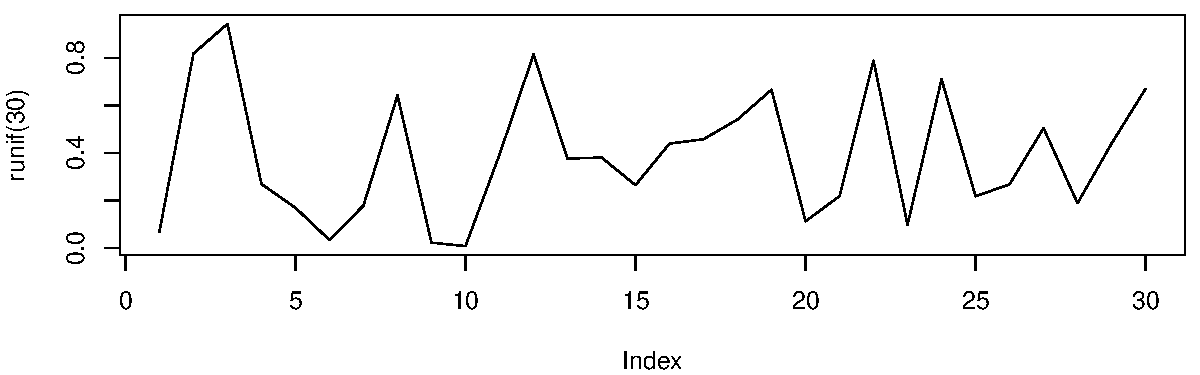
\includegraphics[width=\maxwidth]{figure/ch02_figunnamed-chunk-3-1} 

\end{knitrout}
  \caption{Test figure to illustrate figure options used by knitr.}
  \label{f02:1}
\end{figure}


The focus of this master thesis is on the LMG variable importance metric. The LMG is a metric that is based on variance decomposition. The total $\Rtwo$ of a model is decomposed onto the predictors. Many authors call this a desirable property of a variable importance metric. Marginal and conditional information are incorporated \citep{Gromping2015} .  The following formulas are taken from \cite{Gromping2015}. The same mathematical notations are used. 

The following  notations for the explained variance (1) and sequentially added variance (2) simplify the notation of the LMG formula. 

   \begin{align} 
     \EVAR(S) = \var(Y) - \var( Y \mid X_{j}, j \in S),   \label{eq:1} 
   \end{align} 
   \begin{align} 
     \SVAR(M \mid S) = \EVAR(M \cup S) - \EVAR(S), \label{eq:2} 
    \end{align} , where S and M denote disjoint sets of predictors.
    
   The LMG formula is given below for the first predictor only. Because of exchangeable predictors, this is no loss of generality.  $\Rtwo(S)$ can be written as $\EVAR(S)/\var(Y).$ 

   \begin{align} 
     \LMG(1) &= \frac{1}{p!} \sum_{\pi permutation}^{} \SVAR(\{1\} \mid S_{1}(\pi)),   \nonumber  \\
     &= \frac{1}{p!} \sum_{S \subseteq \{ 2, \dots, p \} }^{} n(S)!(p-n(S)-1)! \SVAR(\{1\} \mid S) \nonumber  \\
     &=  \cfrac{1}{p} \sum_{i=0}^{p-1} \left( \substack {\sum\limits_{ S \subseteq \{ 2, \dots, p \}}\\n(S)=1}^{} \ \SVAR(\{1\} \mid S)\right)\bigg/ \binom{p-1}{i}\\   
         &=  \cfrac{1}{p} \sum_{i=0}^{p-1} \frac{ \substack{\sum\limits_{ S \subseteq \{ 2, \dots, p \}}\\n(S)=1}^{} \ \SVAR(\{1\} \mid S)}{\binom{p-1}{i}} \\      
   \end{align},
   where $S_{1}(\pi)$ is the set of predecessors of predictor 1.
   
   The different writings of the formulas help to better grasp what is calculated in the LMG metric. The $\Rtwo$ of the model including all predictors is decomposed. In the top formula the LMG value of predictor 1 is represented as an unweighted average over all orderings of the sequentiel added variance contribution of predictor 1. The middle formula shows that the calculation can be  done computationally more efficient. The orderings with the same set of predecessors $S$ are combined into one summand. Instead of $p!$ summands only $2^{p-1}$ summands need to be calculated. The bottom formula shows that the LMG metric can also be seen as the unweighted average over average explained variance improvements when adding predictor 1 to a model of size i without predictor 1 \citep{Gromping2015}. 
The LMG metric is implemented in the R package relaimpo .
Chevan and Sutherland propose that instead of only using the variances, an appropriate goodness-of-fit metric can as well be used in the LMG formula. They name their proposal hierarchical partitioning. The requirements are simply: an initial measure of fit when no predictor variable is present, a final measure of fit when N predictor variables are present, all intermediate models when various combinations of predictor variables are present. 
  The LMG component of each variable is named independent component (I). The sum of the independent components (I) results then in the overall goodness-of-fit metric. The difference between the goodness-of-fit when only the predictors itself is included in the model, compared to its independent component (I) is named the joint contribution (J).  When $\Rtwo$ is chosen as the measure of fit the same LMG values as in relaimpo was calculated. However,  the hier.part package is only guaranteed to work for 9 predictors. 

For the linear model the $\Rtwo$ is the most widely used goodness-of-fit metric.  Different formulas for $\Rtwo$ exist \cite{Kvalseth1985}, all leading to the same value when and intercept is included and the model is fitted by maximum likelihood. 

Two popular definitions are:
   
      \begin{align} 
     R^2 &= 1 - \frac{\sum_{i=1}^{n}(y_{i} - \hat{y_{i}})^2}{\sum_{i=1}^{n}(y_{i}-\bar{y})^2}   \label{eq:rtwo1} \\
     R^2 &= \frac{\sum_{i=1}^{n}(\hat{y_{i}} - \bar{y})^2}{\sum_{i=1}^{n}(y_{i}-\bar{y})^2}, \qquad i = 1,\dots,n,   \label{eq:rtwo2} 
   \end{align} 
   
, where $\hat{y_{i}} = = \E ({y \mid X_{i}, \hat{\theta}})$.  $\hat{\theta}$ is the maximum likelihood estimate of the regression coefficients.


When other estimation methods than maximum likelihood are used \eqref{eq:rtwo1} can be negative and \eqref{eq:rtwo2}  can be bigger than 1. This is not uncommon in a Bayesian Regression setting, when samples of the posterior parameter distribution are employed. A model that explaines more than 100\% of the variance does not make sense. A negative $\Rtwo$ is also difficult to interpret. A negative $\Rtwo$ may be interpreted as a fit that is worse than the mean of the data. This can make sense for predictive purposes, e.g. when new data from a test set is predicted by leave-one-out crossvalidation \citep{Alexander2015}.  For non predicting purposes a negative $\Rtwo$ does not make sense. The aim of the LMG formula is to gain some more information about the possible association between variables. A predictor can not explain less than zero variance in the population. To respect the non-negative share property of the LMG formula the $\Rtwo$ of submodels should not decrease when adding predictors. Both classical $\Rtwo$ definitions seem not to be well suited for the LMG metric in the Bayesian framework. Because of $\Rtwo$ bigger than one or the possibility of negative $\Rtwo$ values \cite{Gelman2017} proposes to use:

      \begin{align} 
       \Rtwo_{Gelman} = \frac{\var(\sum_{i=1}^{n}\hat{y}^s_{i})}{\var(\sum_{i=1}^{n}\hat{y}^s_{i})+\var(\sum_{i=1}^{n}e^s_{i})}, \qquad i = 1,\dots,n, \label{rtwoGelman} 
   \end{align} 
   
, where $\hat{y}^s_{i}  = \E \left({y \mid X_{i}, \theta^s}\right) $ and the vector of errors $e^s_{i} = y_{i} - \hat{y}^s_{i}$ and $\theta^s, s = 1, ... , S$ are draws from the posterior parameter distribution. The formula is then guaranteed to be between 0 and 1. The $\Rtwo$ can  be interpreted as a data-based estimate of the proportion of variance explained for new data under the assumption that the predictors are held fixed \citep{Gelman2017}.  However, we can no longer interpret an increase in $\Rtwo$ as a improved fit to a fixed target because the denominator of $\Rtwo$ is no longer fixed . This seems to be problematic for the LMG formula in the Bayesian framework. However, in the linear model it is possible to calculate the $\Rtwo$ of all submodels from the parameters of the fullmodel and the covariance matrix of the predictors. We therefore compare all submodels of a posterior sample to the same fixed value. How it is possible to get the $\Rtwo$ of the submodels from the full model is shown in the next section.


The variance of the linear model can be written as 

      \begin{align} 
        \var(y) = \bbeta^\top \bSigma_{\X \X}  \bbeta + \sigma^2, \label{eq:vary} 
   \end{align}
where $\bbeta^\top = (\beta_{1} \dots \beta_{p})$ are the regression parameters without the intercept.
$\bSigma_{\X \X}$ is the covariance matrix of the regressors.

Writting it this way makes it clear that the predictors in \eqref{rtwoGelman} could also be taken as random \citep{Gelman2017}. The predictors are then called stochastic predictors. We have then an additional uncertainty in the $\Rtwo$ formula that can have a large influence on the $\Rtwo$ values.

In the Bayesian framework the $\sigma^2$ parameter is explicitly modeled in the standard linear regression setting. It is therefor possible to sample the $\sigma^2$ parameter from its posterior distribution instead of defining the error as in \eqref{rtwoGelman}, which woud lead to the following definition:

    \begin{align} 
        R^2 = \frac{\var(\sum_{i=1}^{n}\hat{y}^s_{i})}{\var(\sum_{i=1}^{n}\hat{y}^s_{i})+\sigma^s} \label{rtwoused} 
   \end{align} 
 , where $\hat{y}^s_{i}  = E \left({y \mid X_{i}, \theta^s}\right) $,  and $\theta^s, s = 1, ... , S$ are draws from the posterior parameter distribution.
 
In practice \eqref{rtwoused} and \eqref{rtwoGelman} should lead to  similar values in the standard linear model. In my opionion it is more reasonable to go the full bayesian route and sample  $\sigma^2$. This provides us the opportunity to include prior information abouth $\sigma^2$ directly into to $\Rtwo$ calculations. The LMG calculations in the examples of this master thesis will therefore be based on \eqref{rtwoused}.  The benefit of \eqref{rtwoGelman} is that it also works for generalized linear models, where we often have no separate variance parameter.  


For two predictors \eqref{eq:vary} simplifies to

      \begin{align} 
        \var(y) = \beta_{1}^2 \var(X_{1}) + 2  \beta_{1}  \beta_{2} \cov(X_{1}, X_{2}) + \beta_{2}^2 \var(X_{2}) + \sigma^2, \label{varx1x2} 
   \end{align}
 
 When predictor $X_{1}$ is alone in the model the explained variance includes the variance of the predictor itself, the whole covariance term and in addition some of the contribution of the variance of $X_{2}$ in \eqref{varx1x2} . In mathematical notation that is
 
      \begin{align} 
        \SVAR({X_{1}} \mid \emptyset ) = \beta_{1}^2 \var(X_{1}) + 2  \beta_{1}  \beta_{2} \cov(X_{1}, X_{2}) + \beta_{2}^2 \var(X_{2}) \rho_{12}^2 \nonumber 
   \end{align}
   
The contribution of the second regressor is then simply the difference to the total explained variance. 

In the general case with $p$ regressors, the conditional variance formula \eqref{eq:condvar} can be used to calculate the $\Rtwo$ of all submodels. The conditional variance formula can for example be used to specify the conditional distribution of a multivariate normal distribution $\Y$ .

The elements of the vector $\Y$ are reordered as
\begin{align*}
\mathbf{Y} = \begin{pmatrix}
\mathbf{Y}_{1} \\ 
\mathbf{Y}_{2} \end{pmatrix}, \mathbf{Y}_{1} \in \IR^q, \mathbf{Y}_{2} \in \IR^{p-q} .
\end{align*}

The joint distribution is a multivariate normal distribution with elements
\begin{align*}
\begin{pmatrix}
\mathbf{Y}_{1} \\ 
\mathbf{Y}_{2} \end{pmatrix} \sim \mathcal{N}
\Bigg(\begin{pmatrix}
\boldsymbol{\mu}_{1} \\ 
\boldsymbol{\mu}_{2} 
\end{pmatrix},
\begin{pmatrix}
\bSigma_{11} & \bSigma_{12} \\
\bSigma_{21} & \bSigma_{22} \\
\end{pmatrix}\Bigg),
\ \bSigma_{21} = \bSigma_{12}^{T},
\end{align*}
the conditional distribution is normally distributed again with mean 
\begin{align*}
\E (\mathbf{Y}_{1} | \mathbf{y}_{2} ) = \boldsymbol{\mu}_{1}\ +\ \bSigma_{12} \bSigma_{22}^{-1}(\mathbf{Y}_{2}\ -\ \boldsymbol{\mu}_{2})
\end{align*}
and the conditional variance is
\begin{align}
\var ( \mathbf{Y}_{1} | \mathbf{y}_{2} ) = \bSigma_{11}\ -\ \bSigma_{12} \bSigma_{22}^{-1}\bSigma_{21} \text{.} \label{eq:condvar} 
\end{align}

We want to calculate $\Rtwo$ of a submodel containining the predictors $\X_{q...p}$, and regression coefficients $\bbeta^\top = (\beta_{1}, \dotsc, \beta_{p})$ without the intercept. The regression coefficients are further separated in $\bbeta^\top_{1  ,\dotsc,  q-1} = (\beta_{1} ,\dotsc, \beta_{q-1})$ and $\bbeta^\top_{q ,\dotsc, p} = (\beta_{q} ,\dotsc, \beta_{p})$. 

As in the normal distribution example above we have the covariance matrix of $p$ predictors written as 

      \begin{align*} 
\cov(\X) =	\bSigma_{\X \X} = \begin{pmatrix}
\bSigma_{11} & \bSigma_{12} \\
\bSigma_{21} & \bSigma_{22}  \\
\end{pmatrix}^{p \times p}, 
   \end{align*}
   
         \begin{align*} 
   \text{where} \qquad \bSigma_{11} &= \cov(\X_{1,\dotsc, q-1}, \X_{1 ,\dotsc,q-1}), \\ \bSigma_{12} &= \cov(\X_{1,\dotsc, q-1}, \X_{q ,\dotsc, p}),\\ \bSigma_{22} &= \cov(\X_{q ,\dotsc, p}, \X_{q \dots p}) \text{.} \nonumber
      \end{align*}
      
 The conditional variance of the predictors $ \X_{1 ,\dotsc, q-1} $ given the predictors  $ \X_{q ,\dotsc, p} $ is then
 
          \begin{align*} 
 \cov(\X_{1,\dotsc, q-1} \mid \x_{q ,\dotsc, p}) = \bSigma_{11}\ -\ \bSigma_{12} \bSigma_{22}^{-1}\bSigma_{21} 
       \end{align*}
       
       The total explained variance of the full model $\X_{1 \dots p}$ omits simply the $\sigma^2$ parameter in equation , which is

      \begin{align*} 
        \EVAR(\X_{1 ,\dotsc, p}) = \bbeta^\top \bSigma_{\X \X}  \bbeta. 
   \end{align*}

The explained variance of a submodel can be calculated by subtracting from the total explained variance the explained variance of the not-in-the-model-included-predictors that is not explained by in-the-model-included-predictors. The variance that is not explained by in-the-model-included-predictors is given by the variance of the not-in-the-model-included predictors conditional on the in-the-model-included-predictors. The explained variance of a submodel containing predictors $\X_{q ,\dotsc, p}$ can therefore be written as

       \begin{align} 
       \EVAR(\X_{q \dots p}) =  \EVAR(\X_{1  ,\dotsc, p}) - \bbeta^\top_{1 ,\dotsc, q-1} \cov(\X_{1,\dotsc, {q-1}} \mid \x_{q \dots p}) \bbeta_{1 ,\dotsc, {q-1}} . \label{eq:varsub} 
   \end{align}

To gain the the $\Rtwo$ value of the submodel we need to divide the explained variance by the total variance,
       \begin{align*} 
\EVAR(\X_{q ,\dotsc, p}) / \var(\Y).   
\end{align*}

The LMG formula requires calculation of the $\Rtwo$ values for all $2^p-1$ submodels. 

In the Bayesian setting we do have a whole probability distribution for each regression parameter. We can sample the regression parameters from the posterior joint distribution of the fullmodel and use the conditional variance formula to calculate the explained variance of all submodels for each parameter sample. As Gelman notes their $\Rtwo$ can no longer be interpreted as a fit to a fixed target. For the LMG formula this may be problematic. However, using the conditional variance formula to calculate the $\Rtwo$ of the submodels, the same total variance is used for a sample of the joint posterior distribution. The important property that all shares should be non-negative and the dependence of the submodels to each other is then respected for each sample. With dependence, i mean the interconnection of the $\Rtwo$ values of the submodels. As an example for a violation of this interconnection lets assume we have uncorrelated predictors. Instead of fitting the full model and use the conditional mean formula to get the $\Rtwo$ of the submodels,  it would be possible to fit a separate Bayesian model for each submodel. The LMG values could then be built by sampling a parameter from each submodel. The problem is then that the paramter values change in each submodel, even if the predictors are uncorrelated. We would have many possibly true parameter values of a predictor in the same LMG comparison. It would then also be possible that the $\Rtwo$ decreases when adding predictors.  
A further of fitting one full model only  is that we only need to fit one Bayesian model including all predictors. This makes it possible to calculate the LMG values also in the Bayesian framework in a reasonable amount of time. 


\section{Bayesian Regression}
This Section provides a short introduction Bayesian regression and about some assumptions. It is summarized from the book (Bayesian Analysis for the Social Sciences, 2009). 
In regression analysis we are interested in the dependence of $\y$ on $\X$. The conditional mean of a continuous response variable $\y = (y_{1}, \dots, y_{n})^\top)$ is related to a $n \times k$ predictor matrix $\X$ via a linear model, 

       \begin{align} 
\E(\y \mid \X , \bbeta) = \X \bbeta ,
   \end{align}
where $\bbeta$ is a $k \times 1$ vector of unknown regression coefficients.

Under some assumptions about the density, conditional independence and homoskedastic variances, the regression can be written as

       \begin{align} 
\y \mid \X , \bbeta, \sigma^2 \sim \mathcal{N}(\X \bbeta , \sigma^2 \I_{n})
   \end{align}

Under the assumption of weak exogeneity and conditional indepdendence the joint density of the data can be written as

       \begin{align} 
p(\y, \X \mid \btheta) = p(\y \mid \X, \btheta_{y \mid x}) \, p(\X \mid \btheta_{x}),
   \end{align}

where $\btheta = (\btheta_{y \mid x}, \btheta_{x})^\top$. The weak exogeneity assumption implicates that the whole information about $\y_{i}$ is contained in $x_{i}$ and $\btheta_{y \mid x}$. Knowledge of the parameters $\btheta_{x_{i}}$ provides no additional information about $\y_{i}$.
The interest of regression is mostly in the posterior parameters $\btheta_{y \mid x}$. These posterior densities are proportional to  likelihood of the data  multiplied by the prior densitiy. The joint density $p(\y, \X \mid  \btheta)$ is used to learn about the posterior parameters, via Bayes Rule

       \begin{align} 
p(\btheta \mid \y, \X) \propto p(\y, \X \mid  \btheta) \, p(\btheta).
   \end{align}
   
   The dependence of $\y$ on $\X$ is captured in the parameters $\btheta_{y \mid x} = (\beta, \sigma^2)$. Under the assumption of indepdentent prior densities about $\btheta_{y \mid x}$ and $\btheta_{x}$ the posterior distribution of the parameters can be written as
   
          \begin{align} 
p(\bbeta, \sigma^2, \btheta_{x} \mid \y, \X) = \frac{p(\y \mid \X, \bbeta, \sigma^2) \, p(\bbeta, \sigma^2)}{p(\y \mid \X)} \times \frac{p(\X \mid \btheta_{x}) \, p(\btheta_{x})}{p(\X)}
   \end{align}
   
  This factorization shows that under the above mentioned assumptions the posterior inference about the parameters $\btheta_{y \mid x} = (\beta, \sigma^2)$ is indepdendent from the inference about $\btheta_{x}$ given data $\X$. This also means that the assumptions about $\X$ being fixed or stochastic result in the same posterior density of  $\btheta_{y \mid x}$. In the case of fixed regressors $p(\X)$ and $\btheta_{x}$ drop out of the calculations. For stochastic predictors it means that given $\X$ nothing more can be gained about $\theta_{y \mid x} = (\bbeta, \sigma^2)$ from knowing $\btheta_{x}$. 
  
  In regression the focus is on $\btheta_{y \mid x} = (\bbeta, \sigma^2)$, for which under some assumptions it does not matter whether we assume fixed or stochastic predictors. For the LMG formula the variance of the predictors is also incorporated. The LMG formula may be especially interesting for continuous predictors, which in most cases are stochastic. For stochastic predictors the information about $\btheta_{x}$ would therefore also be relevant.  As seen in equation ... inference about $\btheta_{x}$  is independent from inference about $\btheta_{y \mid x}$. If we have stochastic predictors and ignore dependence we just use an estimate of the covariance matrix and do not incorporate this uncertainty.  Because the explained variance is calculated by $\bbeta^\top \bSigma_{\X \X}  \bbeta$, inference about  $\btheta_{x}$  seems to be equally important as inference about $\btheta_{y \mid x}$ for stochastic predictors. If we know the distribution of the $p(\X)$ the $\btheta_{x}$ could be estimated. However, the computation times are then much higher. We would need to do the whole LMG calculation for each posterior covariance sample of the predictors. Depending on the number of predictors this would quite take some time.  In most cases the problem is that we do not know the distribution of the $\X$. As a practical solution we could then use nonparametric bootstrapping to include the uncertainty of the stochastic predictors in the LMG formula. We would then also need to do the whole LMG caclulations for each bootstrap sample of the covariance matrix. There exist also different covariance estimator. The shrinkage method may be an interesting estimator with some interesting properties. 
  
  
  
 

\bibliographystyle{mywiley} 
\bibliography{biblio}
\end{document}
